\begin{figure*}[!h]
  \centering \Cshadowbox{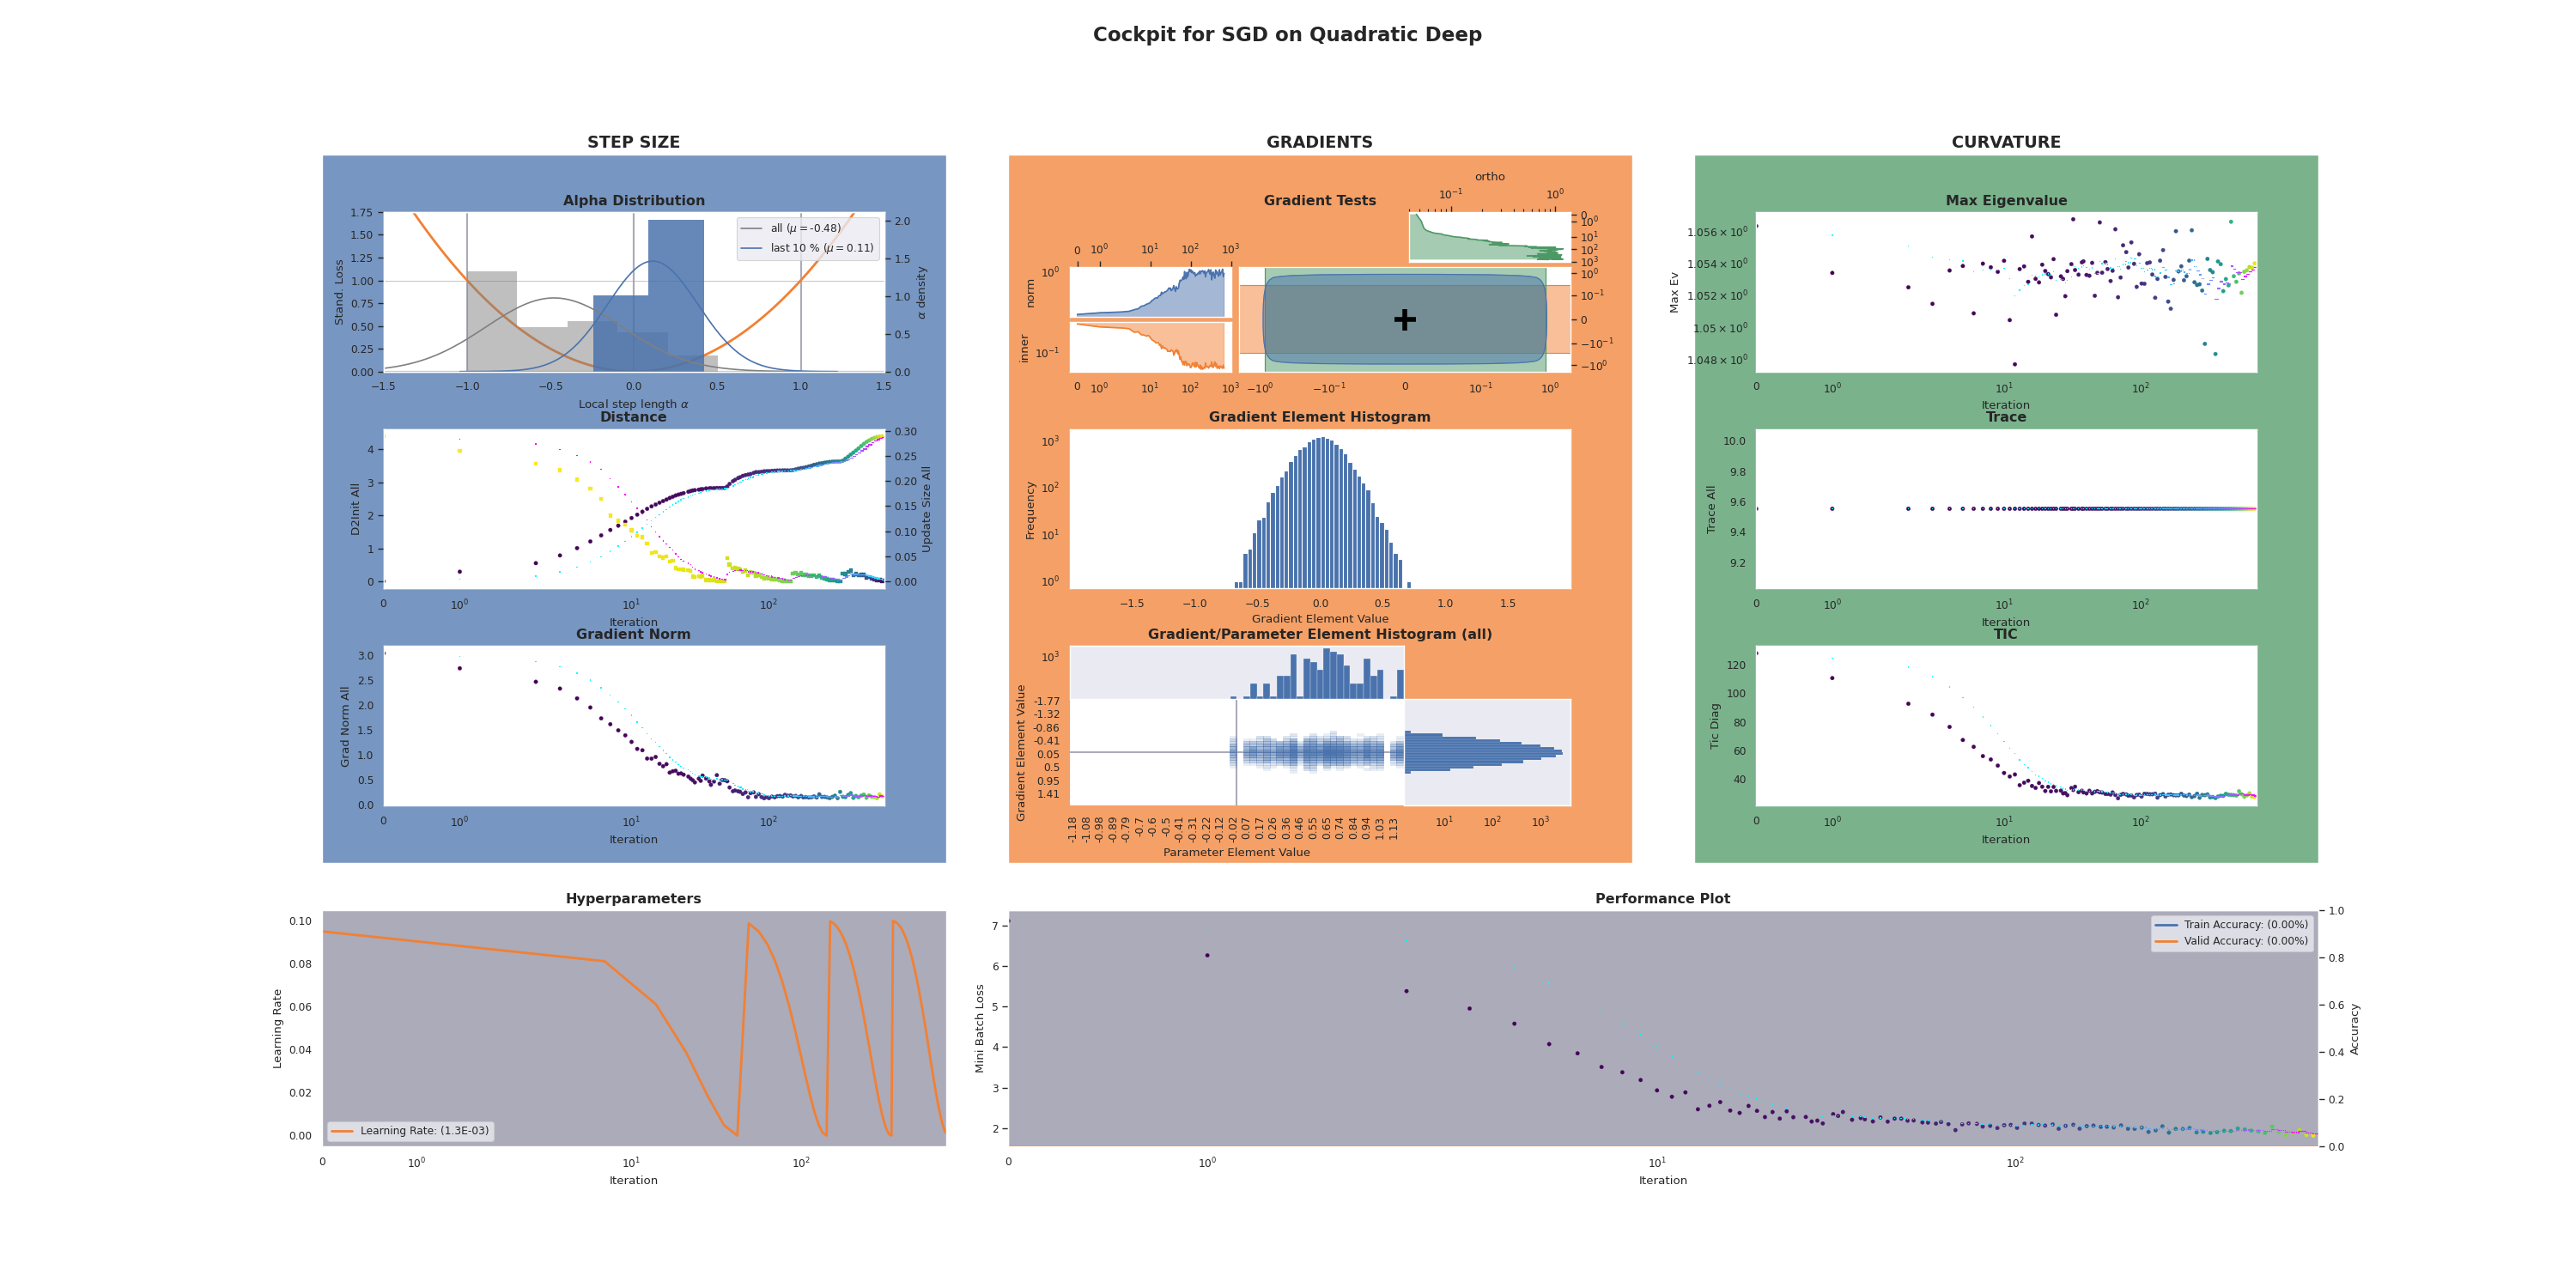
\includegraphics[width=.97\linewidth, trim={7cm 2.5cm
      5cm 0.5cm}, clip]{../repos/cockpit-paper/tex/fig/10_showcase/quadratic_deep_log.png}}

  \Cshadowbox{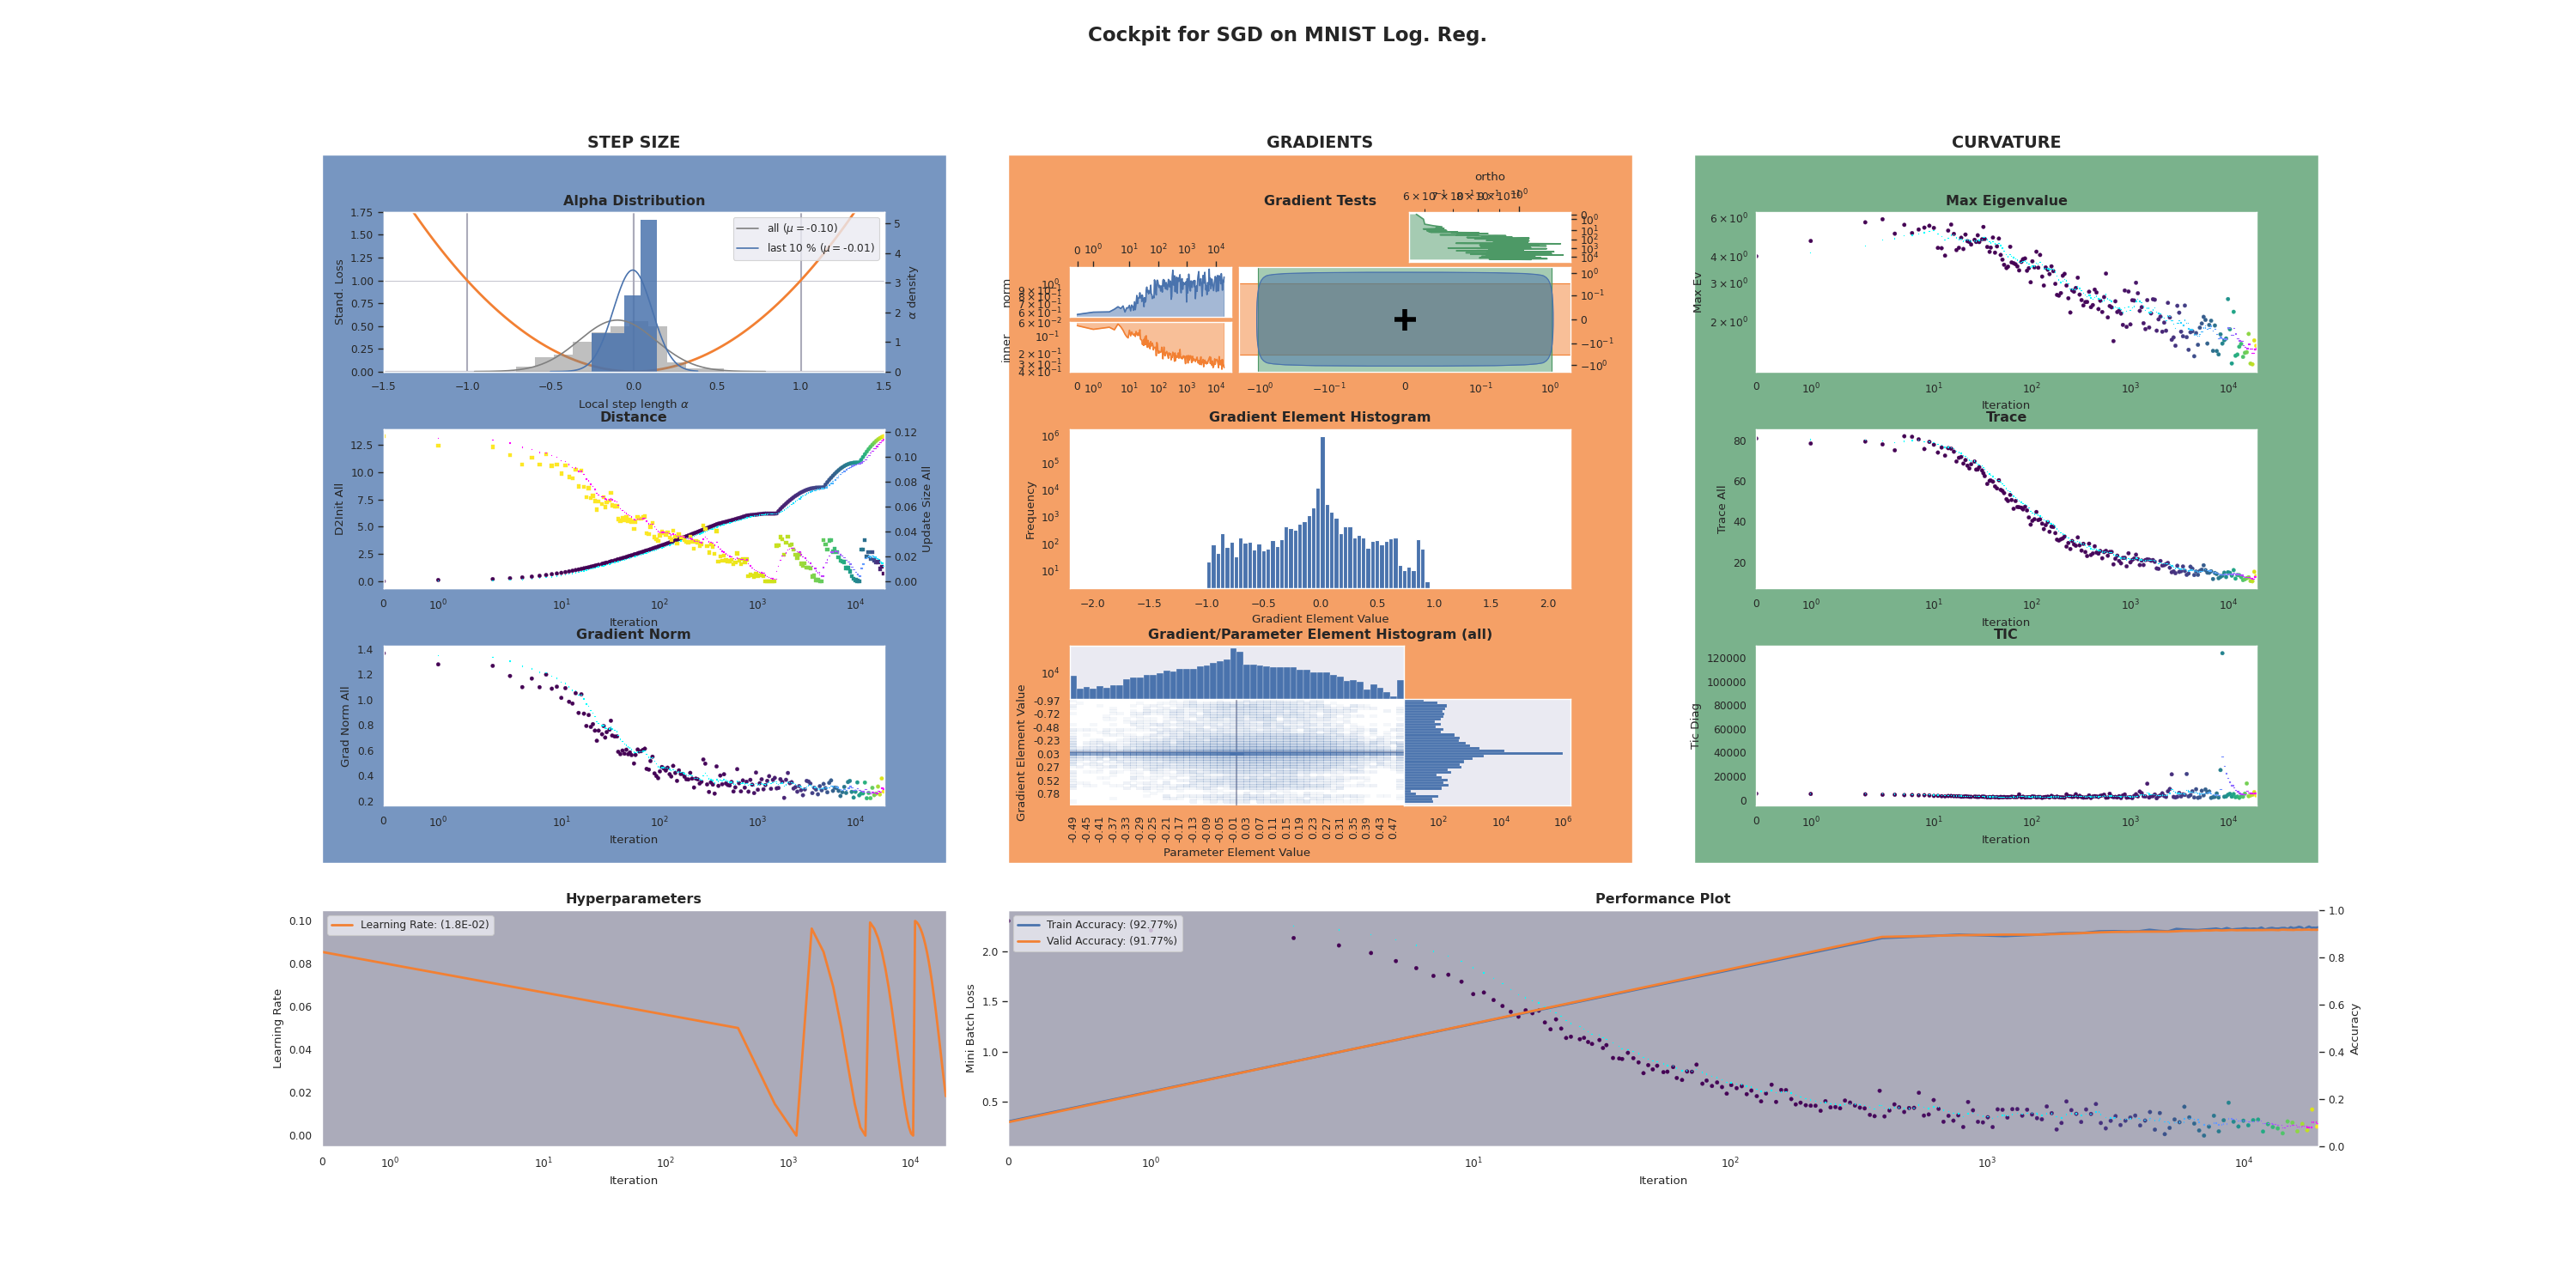
\includegraphics[width=.97\linewidth, trim={7cm 2.5cm 5cm 0.5cm},
    clip]{../repos/cockpit-paper/tex/fig/10_showcase/mnist_logreg_log.png}}

  \vspace{0.5\baselineskip}

  \caption{\textbf{Screenshot of \cockpittitle's full view for convex \deepobs
      problems.} Top \cockpit shows training on a noisy quadratic loss function.
    Bottom shows training on logistic regression on \mnist . Figure and labels
    are not meant to be legible. It is evident, that there is a fundamental
    difference in the optimization process, compared to training deep networks,
    \ie \Cref{cockpit::fig:showcase}. This is, for example, visible when comparing the
    gradient norms, which converge to zero for convex problems but not for deep
    learning.}\label{cockpit::fig:convex-problems}
\end{figure*}

%%% Local Variables:
%%% mode: latex
%%% TeX-master: "../thesis"
%%% End:
